\documentclass[UTF8]{ctexart}

% font packages
\usepackage{amsfonts}
\usepackage{amssymb}
\usepackage{amsthm}
\usepackage{amsmath}
\usepackage{mathrsfs}

% margin
\usepackage{geometry}
\geometry{
    paper =a4paper,
    top =3cm,
    bottom =3cm,
    left=2cm,
    right =2cm
}
\linespread{1.2}

% more math operators' support
\usepackage{physics}

% Boldface
\usepackage{bm}

% Tikz
\usepackage{tikz}
\usetikzlibrary{calc}

% Gaussian Elimination
\usepackage{gauss}

% Commutative Graph
\usepackage[all]{xy}

% Comment
\usepackage{comment}

% Colors
\usepackage{xcolor}

% 文字颜色的命令
\newcommand{\tc}[4][white]{{\fcolorbox{#1}{#2}{\textcolor{#3}{#4}}}} % 此命令接受四个参数,第一个参数为边框颜色,默认为白色,第二个参数为文字背景颜色,第三个参数为文字颜色,第四个参数为文字内容。如:\tc[green]{blue}{lime}{Hello,world!}

% Reference support
\usepackage{hyperref}
\hypersetup{
    colorlinks=true,
    linkcolor=blue,
    filecolor=magenta,
    urlcolor=cyan
} % 请在此处自定义链接的颜色,相当于\textcolor

% Info
\title{Title}
\author{Fulcrum4Math}
\date{\today}

% General
\DeclareMathOperator{\N}{\mathbb{N}}                    % Set of Natural Numbers
\DeclareMathOperator{\Z}{\mathbb{Z}}                    % Set of Integers
\DeclareMathOperator{\Q}{\mathbb{Q}}                    % Set of Rational Numbers
\DeclareMathOperator{\R}{\mathbb{R}}                    % Set of Real Numbers
\DeclareMathOperator{\C}{\mathbb{C}}                    % Set of Complex Numbers

\DeclareMathOperator{\Id}{Id}                           % Identity

\DeclareMathOperator{\Ker}{Ker}                         % Kernel of a Homomorphism ($\ker$ is included in package amsmath)
\DeclareMathOperator{\Image}{Im}                        % Image of a mapping

% Mathematical Logic
\DeclareMathOperator{\true}{\mathbb{T}}                    % Tautology
\DeclareMathOperator{\false}{\mathbb{F}}                    % Contradictory Formula
% Set Theory
\DeclareMathOperator{\PP}{\mathcal{P}}                  % Power Sets
\DeclareMathOperator{\card}{card}                       % Cardinality

% Category Theory
\DeclareMathOperator{\Cat}{\mathcal{C}}                 % Category

\DeclareMathOperator{\Hom}{Hom}                         % Set of Homomorphisms
\DeclareMathOperator{\End}{End}                         % Set of Endomorphisms
\DeclareMathOperator{\Aut}{Aut}                         % Set of Automorphisms
\DeclareMathOperator{\Isom}{Isom}                       % Set of Isomorphisms

\DeclareMathOperator{\Ob}{Ob}                           % Objects of a Category
\DeclareMathOperator{\Mor}{Mor}                         % Morphisms of a Category

% Abstract Algebra

\DeclareMathOperator{\stab}{stab}

% Topology
\DeclareMathOperator{\T}{\mathcal{T}}                   % Topology

\DeclareMathOperator{\intr}{int}                        % Interior
\DeclareMathOperator{\cl}{cl}                           % Closure

\DeclareMathOperator{\U}{\overset{\circ}{\mathit{U}}}   % Deleted Neighbourhood

% Linear Algebra

% \rank is included in package physics.
% \tr is included in package physics.

\DeclareMathOperator{\K}{\mathbb{K}}                    % Number Field
\DeclareMathOperator{\F}{\mathbb{F}}                    % Number Field (F)

\DeclareMathOperator{\diag}{\text{diag}}                % Diagonal Matrix
\DeclareMathOperator{\al}{\bm\alpha}                    % Boldfaced vector alpha
\DeclareMathOperator{\bt}{\bm\beta}                     % Boldfaced vector beta
\DeclareMathOperator{\x}{\bm{x}}                        % Boldfaced vector x
\DeclareMathOperator{\0}{\mathbf{0}}                    % Boldfaced vector x

\newcommand{\Jd}[2]{\mathrm{J}_{#1}{(#2)}}              % Jordan Blocks

% \DeclareMathOperator{\A}{\bm{A}}                    % Boldfaced matrix A
% \DeclareMathOperator{\B}{\bm{B}}                    % Boldfaced matrix B
% \DeclareMathOperator{\Cc}{\bm{C}}                   % Boldfaced matrix C

\DeclareMathOperator{\CCol}{Col}                        % Column Space
\DeclareMathOperator{\RRow}{Row}                        % Row Space
\DeclareMathOperator{\Null}{Null}                       % Null Space
\DeclareMathOperator{\rmT}{\mathrm{T}}                  % Transpose

\newcommand{\spn}{\mathrm{span}\text{ }}             % Span
% The original command `\span` leads to the environment `align` misdirected.

\DeclareMathOperator{\adj}{adj}                         % adj Matrix

\newcommand{\GL}[2]{\mathrm{GL}_{#1}(#2)}               % General Linear Group
\newcommand{\SL}[2]{\mathrm{SL}_{#1}(#2)}               % Special Linear Group

\DeclareMathOperator{\lcm}{lcm}                         % LCM

\newcommand{\<}{\langle}                                
\renewcommand{\>}{\rangle}                              % These two for ordinary Hilbert Inner Products <x,y>
\newcommand{\inprod}[2]{\<#1,#2\>}    % Using $\expval{#1}$ (Included in package physics) can replace \<#1\>.
\newcommand{\ocinterval}[2]{\left(#1,#2\right]}
\newcommand{\cointerval}[2]{\left[#1,#2\right)}
\newcommand{\ccinterval}[2]{\left[#1,#2\right]}
\newcommand{\oointerval}[2]{\left(#1,#2\right)}

% Mathematical Analysis

\DeclareMathOperator*{\ulim}{\overline{\lim}}
\DeclareMathOperator*{\llim}{\underline{\lim}}
\newcommand{\diff}[3]{\left. #1 \right|_{#2}^{#3}}    % This command can be replaced by $\eval{#1}_{#2}^{#3}$ in package physics.

\newcommand{\Ball}[2]{\mathcal{B}\left(#1,#2\right)}	% Open Ball

% Theorem template below copied from https://zhuanlan.zhihu.com/p/763738880

% ————————————————————————————————————自定义颜色————————————————————————————————————
\definecolor{dfn_green1}{RGB}{0, 156, 39} % 深绿
\definecolor{dfn_green2}{RGB}{214, 254, 224} % 浅绿

\definecolor{thm_blue1}{RGB}{0, 91, 156} % 深蓝
\definecolor{thm_blue2}{RGB}{218, 240, 255} % 浅蓝

\definecolor{ppt_pink1}{RGB}{172, 0, 175} % 深粉
\definecolor{ppt_pink2}{RGB}{255, 237, 255} % 浅粉

\definecolor{crl_orange1}{RGB}{225, 124, 0} % 深橙
\definecolor{crl_orange2}{RGB}{255, 235, 210} % 浅橙

\definecolor{xmp_purple1}{RGB}{119, 0, 229} % 深紫
\definecolor{xmp_purple2}{RGB}{239, 223, 255} % 浅紫

\definecolor{cxmp_red1}{RGB}{211, 0, 35} % 深红
\definecolor{cxmp_red2}{RGB}{255, 214, 220} % 浅红

\definecolor{prf_grey1}{RGB}{120, 120, 120} % 深灰
\definecolor{prf_grey2}{RGB}{233, 233, 233} % 浅灰

\definecolor{axm_yellow1}{RGB}{192, 192, 0} % 深黄
\definecolor{axm_yellow2}{RGB}{255, 255, 172} % 浅黄

% 将RGB换为rgb,颜色数值取值范围改为0到1
% ————————————————————————————————————自定义颜色————————————————————————————————————

% ————————————————————————————————————盒子设置————————————————————————————————————

\usepackage{tcolorbox} % 盒子效果
\tcbuselibrary{most} % tcolorbox宏包的设置,详见宏包说明文档

% tolorbox提供了tcolorbox环境,其格式如下:
% 第一种格式:\begin{tcolorbox}[colback=⟨背景色⟩, colframe=⟨框线色⟩, arc=⟨转角弧度半径⟩, boxrule=⟨框线粗⟩]   \end{tcolorbox}
% 其中设置arc=0mm可得到直角;boxrule可换为toprule/bottomrule/leftrule/rightrule可分别设置对应边宽度,但是设置为0mm时仍有细边,若要绘制单边框线推荐使用第二种格式
% 方括号内加上title=⟨标题⟩, titlerule=⟨标题背景线粗⟩, colbacktitle=⟨标题背景线色⟩可为盒子加上标题及其背景线
% 第二种格式:\begin{tcolorbox}[enhanced, colback=⟨背景色⟩, boxrule=0pt, frame hidden, borderline={⟨框线粗⟩}{⟨偏移量⟩}{⟨框线色⟩}]   {\end{tcolorbox}}
% 将borderline换为borderline east/borderline west/borderline north/borderline south可分别为四边添加框线,同一边可以添加多条
% 加入breakable属性可以支持盒子拆分到两页中。
% 偏移量为正值时,框线向盒子内部移动相应距离,负值反之

\newenvironment{dfn_box}{
    \begin{tcolorbox}[enhanced, colback=dfn_green2, boxrule=0pt, frame hidden,
        borderline west={0.7mm}{0.1mm}{dfn_green1},breakable]
    }
    {\end{tcolorbox}}
    
\newenvironment{thm_box}{
    \begin{tcolorbox}[enhanced, colback=thm_blue2, boxrule=0pt, frame hidden,
        borderline west={0.7mm}{0.1mm}{thm_blue1},breakable]
    }
    {\end{tcolorbox}}
    
\newenvironment{ppt_box}{
    \begin{tcolorbox}[enhanced, colback=ppt_pink2, boxrule=0pt, frame hidden,
        borderline west={0.7mm}{0.1mm}{ppt_pink1},breakable]
    }
    {\end{tcolorbox}}
    
\newenvironment{crl_box}{
    \begin{tcolorbox}[enhanced, colback=crl_orange2, boxrule=0pt, frame hidden,
        borderline west={0.7mm}{0.1mm}{crl_orange1},breakable]
    }
    {\end{tcolorbox}}
    
\newenvironment{xmp_box}{
    \begin{tcolorbox}[enhanced, colback=xmp_purple2, boxrule=0pt, frame hidden,
        borderline west={0.7mm}{0.1mm}{xmp_purple1},breakable]
    }
    {\end{tcolorbox}}
    
\newenvironment{cxmp_box}{
    \begin{tcolorbox}[enhanced, colback=cxmp_red2, boxrule=0pt, frame hidden,
        borderline west={0.7mm}{0.1mm}{cxmp_red1},breakable]
    }
    {\end{tcolorbox}}
    
\newenvironment{prf_box}{
    \begin{tcolorbox}[enhanced, colback=prf_grey2, boxrule=0pt, frame hidden,
        borderline west={0.7mm}{0.1mm}{prf_grey1},breakable]
    }
    {\end{tcolorbox}}
    
\newenvironment{axm_box}{
    \begin{tcolorbox}[enhanced, colback=axm_yellow2, boxrule=0pt, frame hidden,
        borderline west={0.7mm}{0.1mm}{axm_yellow1},breakable]
    }
    {\end{tcolorbox}}

% tcolorbox宏包还提供了\tcbox指令,用于生成行内盒子,可制作高光效果

        % \newcommand{\hl}[1]{
        %     \tcbox[on line, arc=0pt, colback=hlan!5!white, colframe=hlan!5!white, boxsep=1pt, left=1pt, right=1pt, top=1.5pt, bottom=1.5pt, boxrule=0pt]
        % {\bfseries \color{hlan}#1}}

% 其中on line将盒子放置在本行(缺失会跳到下一行),boxsep用于控制文本内容和边框的距离,left、right、top、bottom则分别在boxsep的参数的基础上分别控制四边距离

% ————————————————————————————————————盒子设置————————————————————————————————————

% ————————————————————————————————————定理类环境设置————————————————————————————————————
\newtheoremstyle{MyStyle}{0pt}{}{}{\parindent}{\bfseries}{}{1em}{} % 定义新定理风格。格式如下:
%\newtheoremstyle{⟨风格名⟩}
%                {⟨上方间距⟩} % 若留空,则使用默认值
%                {⟨下方间距⟩} % 若留空,则使用默认值
%                {⟨主体字体⟩} % 如 \itshape
%                {⟨缩进长度⟩} % 若留空,则无缩进;可以使用 \parindent 进行正常段落缩进
%                {⟨定理头字体⟩} % 如 \bfseries
%                {⟨定理头后的标点符号⟩} % 如点号、冒号
%                {⟨定理头后的间距⟩} % 不可留空,若设置为 { },则表示正常词间间距;若设置为 {\newline},则环境内容开启新行
%                {⟨定理头格式指定⟩} % 一般留空
% 定理风格决定着由 \newtheorem 定义的环境的具体格式,有三种定理风格是预定义的,它们分别是:
% plain: 环境内容使用意大利斜体,环境上下方添加额外间距
% definition: 环境内容使用罗马正体,环境上下方添加额外间距
% remark: 环境内容使用罗马正体,环境上下方不添加额外间距

\theoremstyle{MyStyle} % 设置定理风格 

% 定义定义环境,格式为\newtheorem{⟨环境名⟩}{⟨定理头文本⟩}[⟨上级计数器⟩]或\newtheorem{⟨环境名⟩}[⟨共享计数器⟩]{⟨定理头文本⟩},其变体\newtheorem*不带编号

% 以下的每个环境接受参数,请按顺序填入:
% #1 环境标题(中文)

\newtheorem{axiom}{公理}[section]
\newenvironment{axm}[2]
{
    \begin{axm_box}
        \begin{axiom}
            \textbf{#1
                \ifx\relax#2\relax\else % 检查 #2 是否为空
                    (#2) % 如果 #2 不为空,渲染 [空格](#2)
                \fi}
            \newline
}
{
        \end{axiom}
    \end{axm_box}
}

\newtheorem{definition}{定义}[subsection]
\newenvironment{dfn}[2]
{
    \begin{dfn_box}
        \begin{definition}
            \textbf{#1
                \ifx\relax#2\relax\else % 检查 #2 是否为空
                    (#2) % 如果 #2 不为空,渲染 [空格](#2)
                \fi}
            \newline
}
{
        \end{definition}
    \end{dfn_box}
}

\newtheorem{concept}[definition]{概念}
\newenvironment{cpt}[1]
{
    \begin{dfn_box}
        \begin{concept}
            \textbf{#1}
            \newline
}
{
        \end{concept}
    \end{dfn_box}
}

\newtheorem{syntax}[definition]{语法}
\newenvironment{syn}[1]
{
    \begin{thm_box}
        \begin{syntax}
            \textbf{#1}
            \newline
}
{
        \end{syntax}
    \end{thm_box}
}

\newtheorem{theorem}[definition]{定理}
\newenvironment{thm}[2]
{
    \begin{thm_box}
        \begin{theorem}
            \textbf{#1
                \ifx\relax#2\relax\else % 检查 #2 是否为空
                    (#2) % 如果 #2 不为空,渲染 [空格](#2)
                \fi}
            \newline
}
{
        \end{theorem}
    \end{thm_box}
}

\newtheorem{mytactic}{策略}
\newenvironment{tactic}[1]
{
    \begin{thm_box}
        \begin{mytactic}
            \textbf{#1}
            \newline
}
{
        \end{mytactic}
    \end{thm_box}
}

\newtheorem{myvariation}{Tactic 变体}[definition]
\newenvironment{tacticvar}[1]
{
    \begin{ppt_box}
        \begin{myvariation}
            \textbf{#1}
            \newline
}
{
        \end{myvariation}
    \end{ppt_box}
}

\newtheorem{example}{ 例\, }[subsection]
\newenvironment{xmp}[1]
{
    \begin{xmp_box}
        \begin{example}
            \textbf{#1}
            \newline
}
{
        \end{example}
    \end{xmp_box}
}

\newtheorem{cexample}{反例}[subsection]
\newenvironment{cxmp}[1]
{
    \begin{cxmp_box}
        \begin{cexample}
            \textbf{#1}
            \newline
}
{
        \end{cexample}
    \end{cxmp_box}
}

\newtheorem*{myproof}{证明: \newline}
\newenvironment{prf}{\begin{prf_box}\begin{myproof}}{\end{myproof}\end{prf_box}}

\newenvironment{crs}[4]
{
    \begin{thm_box}
        \textbf{课程 #1: #2}
        
        \ifx\relax#3\relax\else % 检查 #3 是否为空
            \textbf{主讲: }#3 % 如果 #3 不为空,渲染 [空格](#3)
        \fi
        
        \ifx\relax#4\relax\else % 检查 #4 是否为空
            \textbf{课程材料: }#4 % 如果 #4 不为空,渲染 [空格](#4)
        \fi

        \textbf{主要内容: }
}
{
    \end{thm_box}
}

\newtheorem{project}{课题}
\newenvironment{prj}[1]
{
    \begin{xmp_box}
        \begin{project}
            \textbf{#1}
            \newline
}
{
        \end{project}
    \end{xmp_box}
}

\usepackage{listings}
\newcommand{\smallsec}[1]{\paragraph{#1.}}
\lstset{
    basicstyle = \ttfamily,
}

% Define Colors: 
\definecolor{leanblue}{RGB}{0,0,255}
\colorlet{keyword}{leanblue}
\colorlet{punct}{leanblue}

\definecolor{sorry}{RGB}{255,0,0}
\definecolor{comment}{RGB}{0,128,0}
\definecolor{string}{RGB}{163,21,21}
\definecolor{num}{RGB}{9,134,88}

\definecolor{thname}{RGB}{121,94,38}

\definecolor{background}{HTML}{EEEEEE}
\definecolor{delim}{RGB}{20,105,176}

\newcommand*{\lean}[1]{\texttt{\color{blue}#1}}

\lstdefinelanguage{lean}{
    % Define Keywords: 
    alsoletter = {\#},
    keywords = {
        import, 
        namespace, 
        open, 
        variable, 
        Prop, 
        Type, 
        % Declarations: 
        protected, 
        class, 
        instance, 
        def, 
        axiom, 
        example, 
        theorem, 
        lemma, 
        fun, 
        by, 
        % Basics: 
        \#check, 
        \#leansearch, 
        \#eval, 
        % Tactics: 
        exact, 
            % FOL: 
            intro,
            intros, 
            rintro, 
            apply,
            apply?, 
            constructor, 
            rcases, 
            obtain, 
            use, 
            left, 
            right, 
            cases, 
            case, 
            by\_cases, 
            by\_contra, 
            contrapose, 
            contrapose!,
            % Others: 
            symm, 
            calc, 
            unfold, 
            have, 
            let, 
            rw, 
            at, 
            change, 
            show, 
        }, 
    keywords = [2]{sorry}, 
    %
    numbers=left,
    numberstyle=\color{num},
    %
    % morecomment = [l]{--},
    moredelim=[l][\color{comment}]{--}, % morecomment -> moredelim, so that Unicode characters can be used in comments. 
    moredelim=[is][\color{thname}]{\#tm\{}{\}}, 
    morecomment = [s]{/-}{-/},
    commentstyle = \color{comment}, 
    %
    stringstyle = \color{string}, 
    %
    stepnumber=1,
    numbersep=8pt,
    showstringspaces=false,
    breaklines=true,
    frame=lines,
    backgroundcolor=\color{background},
    literate=
    % Keywords
        {th\_name}{{{\color{thname}th\_name}}}{7}
    % Math Symbols
        {ℕ}{{\ensuremath{\mathbb{N}}}}{1}
        {ℤ}{{\ensuremath{\mathbb{Z}}}}{1}
        {ℝ}{{\ensuremath{\mathbb{R}}}}{1}
        {ℚ}{{\ensuremath{\mathbb{Q}}}}{1}
        {ℂ}{{\ensuremath{\mathbb{C}}}}{1}
        {∩}{{\ensuremath{\cap}}}{1}
        {∪}{{\ensuremath{\cup}}}{1}
        {⊂}{{\ensuremath{\subseteq}}}{1}
        {⊆}{{\ensuremath{\subseteq}}}{1}
        {⊄}{{\ensuremath{\nsubseteq}}}{1}
        {⊈}{{\ensuremath{\nsubseteq}}}{1}
        {⊃}{{\ensuremath{\supseteq}}}{1}
        {⊇}{{\ensuremath{\supseteq}}}{1}
        {⊅}{{\ensuremath{\nsupseteq}}}{1}
        {⊉}{{\ensuremath{\nsupseteq}}}{1}
        {∈}{{\ensuremath{\in}}}{1}
        {∉}{{\ensuremath{\notin}}}{1}
        {∋}{{\ensuremath{\ni}}}{1}
        {∌}{{\ensuremath{\notni}}}{1}
        {∅}{{\ensuremath{\emptyset}}}{1}
        {∫}{{\ensuremath{\int}}}{1}
        {∑}{{\ensuremath{\mathrm{\Sigma}}}}{1}
        {Π}{{\ensuremath{\mathrm{\Pi}}}}{1}
        {≤}{{\ensuremath{\leq}}}{1}
        {≥}{{\ensuremath{\geq}}}{1}
        {≠}{{\ensuremath{\neq}}}{1}
        {≈}{{\ensuremath{\approx}}}{1}
        {≡}{{\ensuremath{\equiv}}}{1}
        {≃}{{\ensuremath{\simeq}}}{1}
    % Greek Letters lowercase
        {α}{{\ensuremath{\mathrm{\alpha}}}}{1}
        {β}{{\ensuremath{\mathrm{\beta}}}}{1}
        {γ}{{\ensuremath{\mathrm{\gamma}}}}{1}
        {δ}{{\ensuremath{\mathrm{\delta}}}}{1}
        {ε}{{\ensuremath{\mathrm{\varepsilon}}}}{1}
        {ζ}{{\ensuremath{\mathrm{\zeta}}}}{1}
        {η}{{\ensuremath{\mathrm{\eta}}}}{1}
        {θ}{{\ensuremath{\mathrm{\theta}}}}{1}
        {ι}{{\ensuremath{\mathrm{\iota}}}}{1}
        {κ}{{\ensuremath{\mathrm{\kappa}}}}{1}
        {μ}{{\ensuremath{\mathrm{\mu}}}}{1}
        {ν}{{\ensuremath{\mathrm{\nu}}}}{1}
        {ξ}{{\ensuremath{\mathrm{\xi}}}}{1}
        {π}{{\ensuremath{\mathrm{\mathnormal{\pi}}}}}{1}
        {ρ}{{\ensuremath{\mathrm{\rho}}}}{1}
        {σ}{{\ensuremath{\mathrm{\sigma}}}}{1}
        {τ}{{\ensuremath{\mathrm{\tau}}}}{1}
        {φ}{{\ensuremath{\mathrm{\varphi}}}}{1}
        {χ}{{\ensuremath{\mathrm{\chi}}}}{1}
        {ψ}{{\ensuremath{\mathrm{\psi}}}}{1}
        {ω}{{\ensuremath{\mathrm{\omega}}}}{1}
    % Greek Letters UPPERCASE
        {Γ}{{\ensuremath{\mathrm{\Gamma}}}}{1}
        {Δ}{{\ensuremath{\mathrm{\Delta}}}}{1}
        {Θ}{{\ensuremath{\mathrm{\Theta}}}}{1}
        {Λ}{{\ensuremath{\mathrm{\Lambda}}}}{1}
        {Σ}{{\ensuremath{\mathrm{\Sigma}}}}{1}
        {Φ}{{\ensuremath{\mathrm{\Phi}}}}{1}
        {Ξ}{{\ensuremath{\mathrm{\Xi}}}}{1}
        {Ψ}{{\ensuremath{\mathrm{\Psi}}}}{1}
        {Ω}{{\ensuremath{\mathrm{\Omega}}}}{1}
    % Arrows
        {↦}{{\ensuremath{\mapsto}}}{1}
        {←}{{\ensuremath{\leftarrow}}}{1}
        {<-}{{\ensuremath{\leftarrow}}}{1}
        {→}{{\ensuremath{\rightarrow}}}{1}
        {->}{{\ensuremath{\rightarrow}}}{1}
        {↔}{{\ensuremath{\leftrightarrow}}}{1}
        {<->}{{\ensuremath{\leftrightarrow}}}{1}
        {⇒}{{\ensuremath{\Rightarrow}}}{1}
        {⟹}{{\ensuremath{\Longrightarrow}}}{1}
        {⇐}{{\ensuremath{\Leftarrow}}}{1}
        {⟸}{{\ensuremath{\Longleftarrow}}}{1}
        {Σ}{{\ensuremath{\Sigma}}}{1}
        {Π}{{\ensuremath{\Pi}}}{1}
        {∀}{{\ensuremath{\forall}}}{1}
        {∃}{{\ensuremath{\exists}}}{1}
        {λ}{{\ensuremath{\mathrm{\lambda}}}}{1}
        {∧}{{\ensuremath{\wedge}}}{1}
        {∨}{{\ensuremath{\vee}}}{1}
        {¬}{{\ensuremath{\neg}}}{1}
        {⊢}{{\ensuremath{\vdash}}}{1}
        {‖}{{\ensuremath{\|}}}{1}
    % subscripts
        {₁}{{\ensuremath{_1}}}{1}
        {₂}{{\ensuremath{_2}}}{1}
        {₃}{{\ensuremath{_3}}}{1}
        {₄}{{\ensuremath{_4}}}{1}
        {₅}{{\ensuremath{_5}}}{1}
        {₆}{{\ensuremath{_6}}}{1}
        {₇}{{\ensuremath{_7}}}{1}
        {₈}{{\ensuremath{_8}}}{1}
        {₉}{{\ensuremath{_9}}}{1}
        {₀}{{\ensuremath{_0}}}{1}
        {ᵢ}{{\ensuremath{_i}}}{1}
        {ⱼ}{{\ensuremath{_j}}}{1}
        {ₐ}{{\ensuremath{_a}}}{1}
        {⁻¹}{{\ensuremath{^{-1}}}}{1}
        {¹}{{\ensuremath{^1}}}{1}
        {ₙ}{{\ensuremath{_n}}}{1}
        {ₘ}{{\ensuremath{_m}}}{1}
        {ₚ}{{\ensuremath{_p}}}{1}
        {ᶜ}{{\ensuremath{^{\mathrm{C}}}}}{1}
    % Others
        {↑}{{\ensuremath{\uparrow}}}{1}
        {↓}{{\ensuremath{\downarrow}}}{1}
        {⊢}{{\ensuremath{\vdash}}}{1}
        {|-}{{\ensuremath{\vdash}}}{1}
        {⊥}{{\ensuremath{\perp}}}{1}
        {∞}{{\ensuremath{\infty}}}{1}
        {∂}{{\ensuremath{\partial}}}{1}
        {√}{{\ensuremath{\sqrt}}}{1}
        {∘}{{\ensuremath{\circ}}}{1}
        {×}{{\ensuremath{\times}}}{1}
        {∆}{{\ensuremath{\triangle}}}{1}
        {⟨}{{\ensuremath{\color{leanblue}\langle}}}{1}
        {⟩}{{\ensuremath{\color{leanblue}\rangle}}}{1}
        {⦃}{{\ensuremath{\color{leanblue}\{\!\mid}}}{1}
        {⦄}{{\ensuremath{\color{leanblue}\mid\!\}}}}{1}
        {ℒ}{{\ensuremath{\mathscr{L}}}}{1}
        {𝒫}{{\ensuremath{\mathcal{P}}}}{1}
        {·}{{\ensuremath{\cdot}}}{1},
}

\lstdefinestyle{lean}{
    language=lean,
    numbers=none, 
    keywordstyle=\color{leanblue},
    keywordstyle=[2]\color{sorry},
    % frame=none,
    backgroundcolor=\color{white}, 
}

\newcommand{\Goal}{\texttt{\,\color{leanblue}\ensuremath{\vdash}\,}}


\begin{document}

    \begin{center}
        {\LARGE\textbf{2025 Lean 与数学形式化讲义(1B)}}

        上海交通大学 AI4MATH 团队
    \end{center}

    \section{初识 Lean}

        我们现在要初步地探索 Lean 交互式形式化定理证明器这一强大工具. 我们不妨先简单体验一下使用 Lean 进行形式化数学证明的感受. 我们会在之后逐步深入探索背后的原理和工作细节. 

    \subsection{认识 Lean 的 VS Code 界面}

        使用 VS Code 编辑器打开 Mathematics In Lean 项目, 定位至以下位置: 

        \texttt{mathematics\_in\_lean/MIL/C01\_Introduction/S02\_Overview.lean}

        \begin{figure}[htbp]
            \centering
            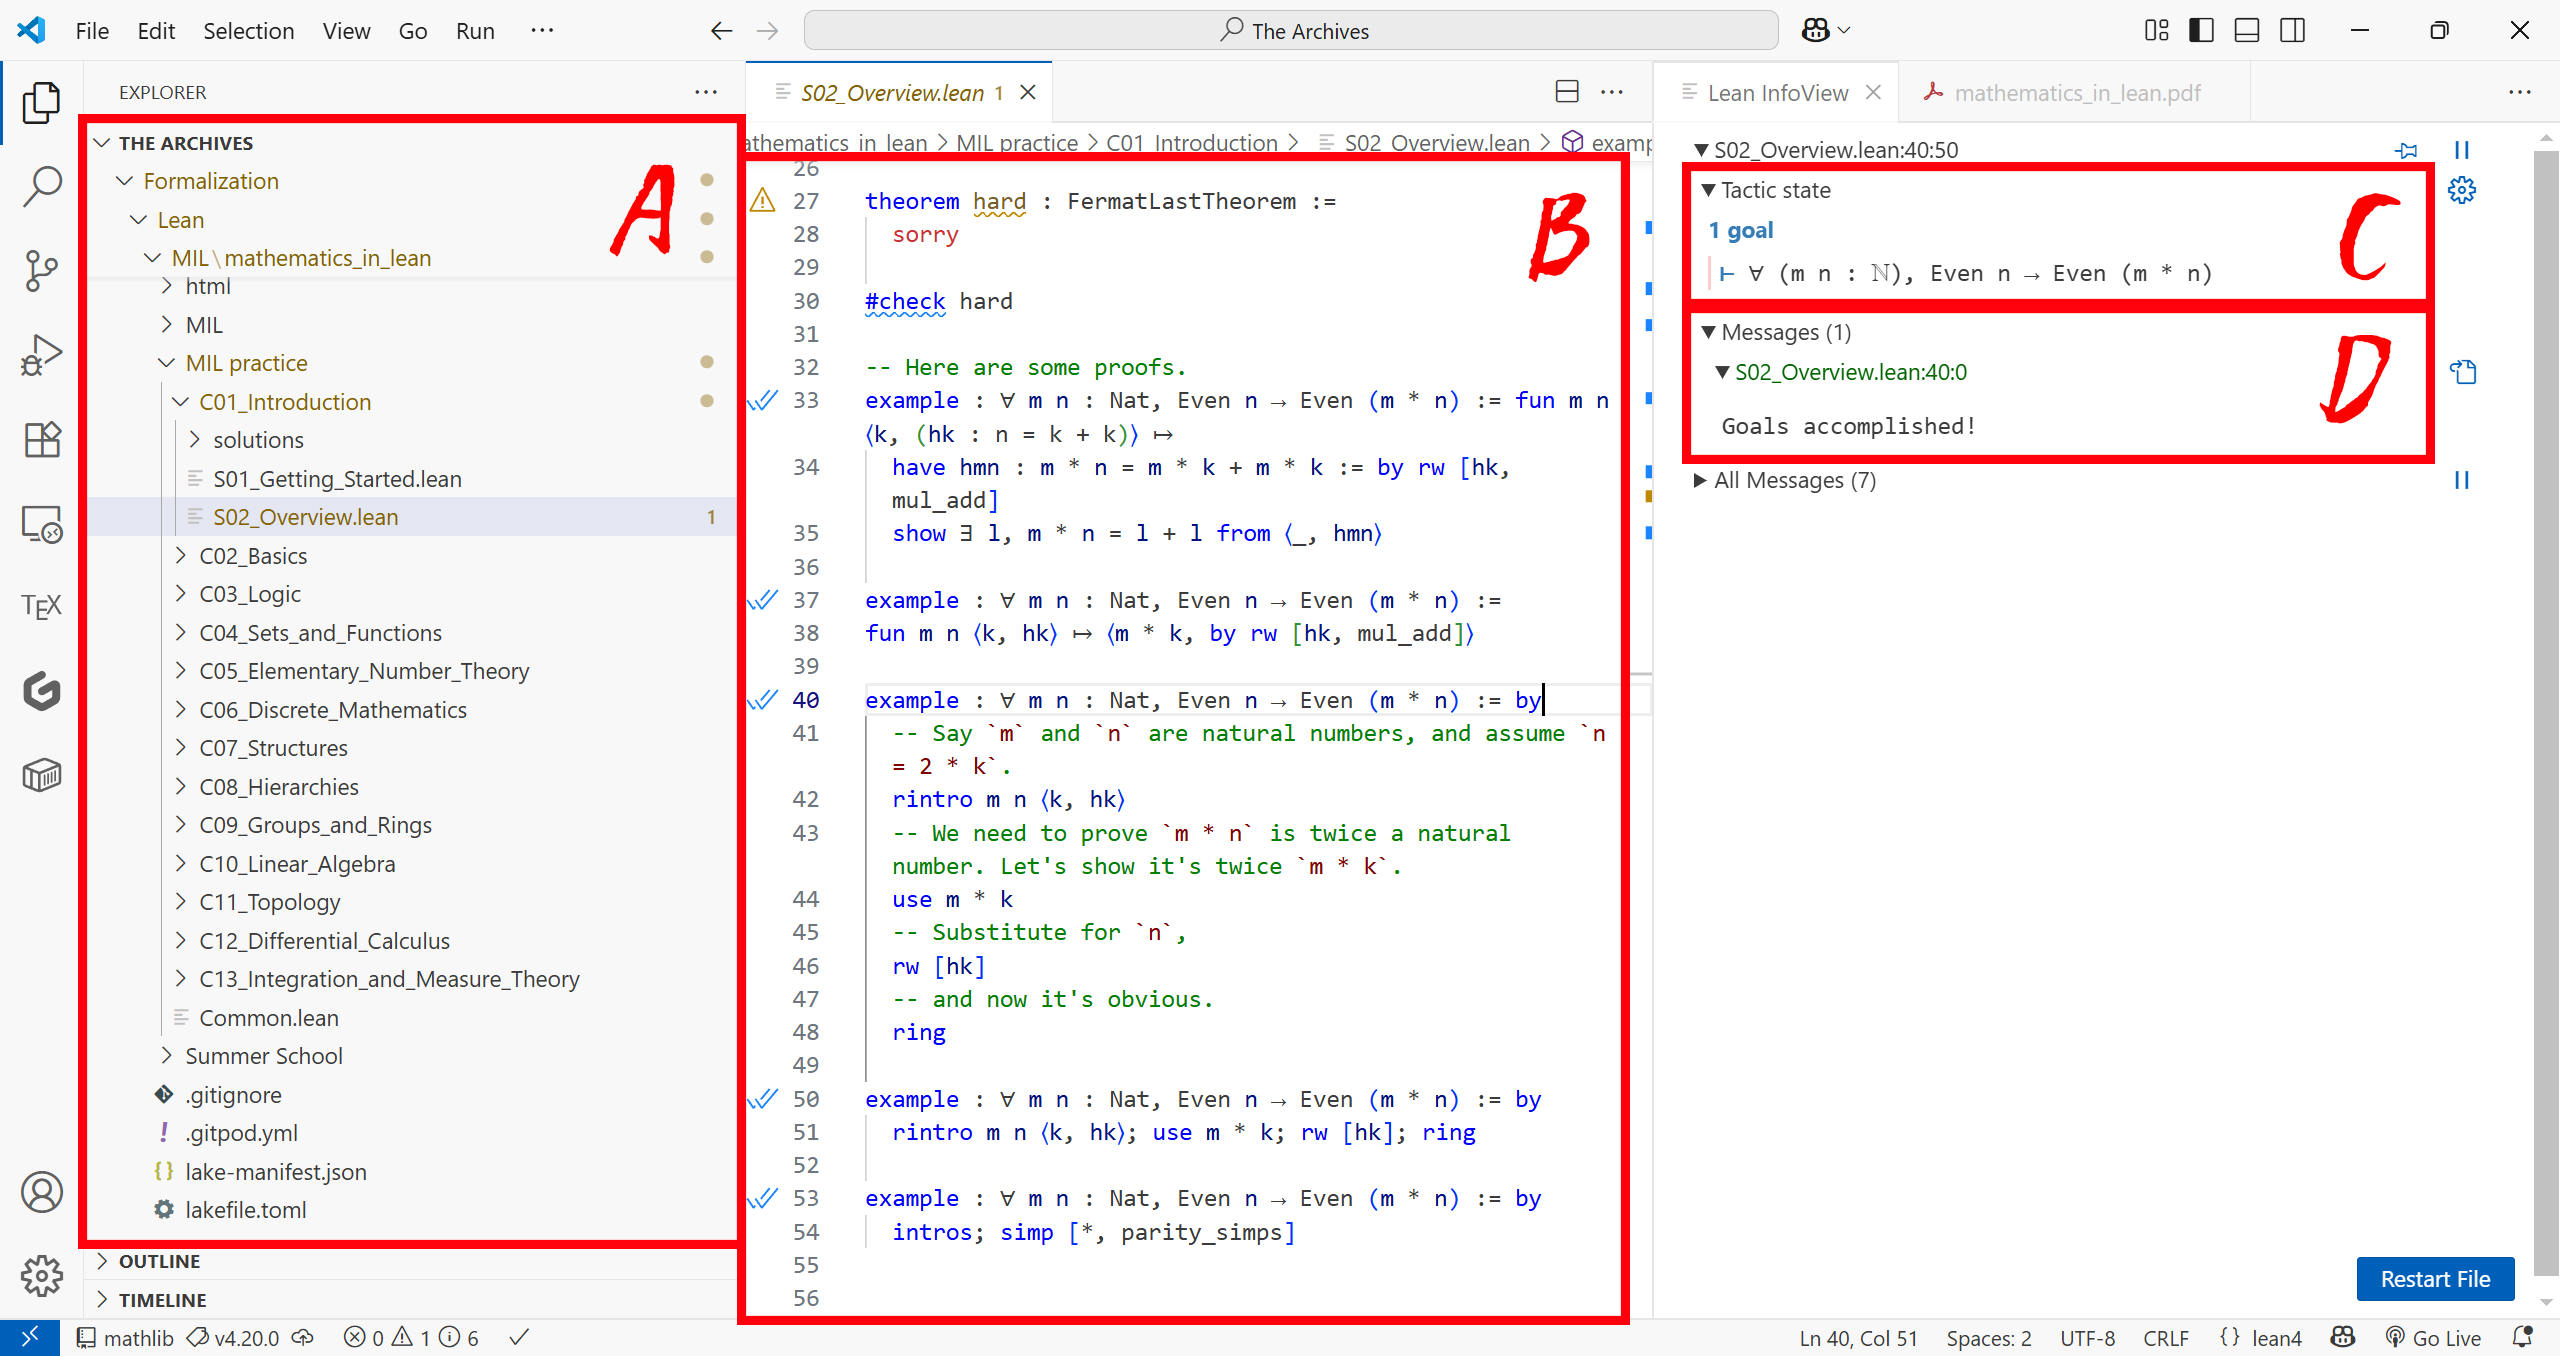
\includegraphics[width=0.8\textwidth]{figures/png/1.png}\label{fig:example1}
            \caption{使用 VS Code 编辑器编写 Lean 的界面}
        \end{figure}
    
        如图\ref{fig:example1}所示, 默认布局下, 界面将以三大纵栏呈现. \footnote{鉴于并非所有人都足够熟悉 VS Code 编辑器, 我们也简作介绍, 同时进行一些术语的统一. }
        
        第一纵栏, 即图中 A 区域, 是 VS Code 自带的\textbf{文件浏览器 (File Explorer)}. 通常我们会打开一个 Lean 项目所在根目录, 并通过文件浏览器来定位至所需查看或编辑的文件. 
        
        第二纵栏, 即图中 B 区域, 是 VS Code 自带的\textbf{代码编辑器 (Code Editor)}. 使用者操作 Lean 工具的方式是使用 Lean 语言编写代码. 

        第三纵栏, 是 VS Code Lean 4 语言扩展提供的功能, 称为 \textbf{Lean 信息视图 (Lean InfoView)}, 主要用于展示 Lean 程序内核通过\textbf{语言服务器协议 (\underline{L}anguage \underline{S}erver \underline{P}rotocol (LSP))}返回给使用者的各类信息. 其中 D 区域是一个常驻栏目, 用于展示任何对应当前光标位置的\textbf{消息 (Messages)}. 特别地, 图中 C 区域依据光标所在位置的语境将展示特别的信息: 在进行定理的形式化证明时, 将展示当前定理的\textbf{证明状态 (Proof State / Tactic State)}; 当进行对象的类型检查时, 将展示被检查对象的类型; 当进行定理检索时, 将展示检索结果或是推荐的下一步证明步骤, 等等. 
        
        现在在 \texttt{mathematics\_in\_lean} 文件夹下新建一个 \texttt{test} 文件夹, 在其中新建一个 \texttt{test.lean} 文件, 并输入以下代码来导入 Mathlib 库 (这可能会比较慢, 建议每节课前先完成这一步): 
        \begin{lstlisting}[style=lean]
    import Mathlib
        \end{lstlisting}

    \subsection{初识类型论}
        
        Lean 依赖的形式化理论框架是\textbf{依值类型论 / 依赖类型论 (\underline{D}ependent \underline{T}ype \underline{T}heory (DTT))}, 简称\textbf{类型论 (Type Theory)}. \footnote{严格来讲, Lean 中并不是所有东西都以类型论为基础, 但这是个很复杂的问题. } 我们在正式上手使用 Lean 之前, 先学习一些简单的类型论\footnote{``简单的依值类型论知识'', 不是 Russell 先生的``简单类型论''. }概念. 请注意, 这只是在初步建立一种``直觉性''的认识, 在第三章的学习中我们会进行更为系统的学习. 

        % 我们不妨想象, 在生活中, 为了向一个刚刚开始认识世界的懵懂孩子描述清楚一个他不明白的事物——比如一只狸花猫——我们要想办法通过一些他已然明白的事物和逻辑关系组装出``狸花猫''. 比如孩子可能已经明白什么是``猫'', 以及``黑色'', ``灰色''等颜色概念. 但是自然语言常常会陷入某种``循环描述'', 字词的语义往往以复杂的方式相互依赖, 这也是现在大语言模型的思想来源之一. 长大后, 我们也许会进行一些哲学的思考, 对每一件事物追问``是什么'', 试图用某种更加本质的东西来解释它们, 直到我们追问至某种先验的存在, 以至于我们再难以提炼出它们的抽象本质. 也许哲学家们有各有不同的理论来解决这些事, 不过在一门数学语言中, 我们不希望出现这种循环描述, 不然很容易 Russell 悖论这样的自指陷阱之中. 类型论就是这样一门强调任何数学对象总是能用某种更原本, 更抽象的数学对象来描述的数学语言. 
        
        
        \begin{cpt}
            {对象的类型 (Type of an Object)}
            在类型论语言下, 任何\textbf{对象 (Object)} 有其\textbf{类型 (Type)}. 
            
            若对象 $a$ 的类型为 $A$, 记作 $a : A$. 
            
            此时称对象 $a$ 是类型 $A$ 的一个\textbf{元素 / 实例 / 项 (Element / Instance / Term)}. \footnote{这个术语很麻烦, 称``元素''容易与``集合-元素''混淆, ``实例''容易与``类-实例''混淆, ``项''则没有强调对象相对其类型的关系. }
        \end{cpt}
        
        \begin{syn}
            {类型检查 (Type Check)}
            在 Lean 中, 使用 \lean{\#check} 命令可以在 InfoView 中查看一个对象的类型. 设 $a : A$, 那么: 
            \begin{lstlisting}[style=lean]
    #check a       --  A
            \end{lstlisting}
        \end{syn}

        我们上述讨论的``对象'', 是类型论语言框架之内被描述的``对象''. 而 Lean 本身作为一个面向``对象''编程得到的程序, 许多``对象''是程序意义下的``对象'', 而非类型论语言描述的``对象''. 这通常包括: 

        \begin{cxmp}
            {Lean 作为元语言自身的语法成分}
            如 \lean{\#check} 命令本身. 查看 ``\lean{\#check}''\footnote{这里的引号不代表字符串. 由于 Lean 同时可承担编程语言的身份, 对字符串进行类型检查是合法的, 结果为 ``\texttt{String}''. } 命令的类型是没有意义的, 只会报错: 
            \begin{lstlisting}[style=lean]
    #check #check  --  error
            \end{lstlisting}
        \end{cxmp}

        \begin{cxmp}
            {类型论作为元语言自身的语法组成部分}
            事实上可归为上一类. 但由于它通常和类型论语言所描述的对象一起出现, 可能更容易引起混淆. 这包括用于类型声明的冒号 ``\texttt{:}'', 定义号 ``\texttt{:=}'' 等等. 查看 ``\texttt{:}'', ``\texttt{:=}'' 的类型也是没有意义的: 
            \begin{lstlisting}[style=lean]
    #check :       --  error
    #check :=      --  error
            \end{lstlisting}
        \end{cxmp}

        \begin{cxmp}
            {Lean 的``语法糖''}
            主要指 Lean 中为了方便人理解而通过 Unicode 符号来表示函数的机制. 例如用加号 ``\texttt{+}'' 指代 ``\texttt{Add}'' 函数\footnote{实际上是某种为了处理符号运算而定义的类型类的实例, 距离具体的函数实现还要再套几层. 这是个很麻烦的问题. }等等. 查看 ``\texttt{+}'' 的类型会报错, 但可以查看 ``\texttt{Add}'' 函数的类型. 
            \begin{lstlisting}[style=lean]
    #check +       --  error
    #check Add     --  Type u -> Type u
            \end{lstlisting}
        \end{cxmp}

        可能还有很多其他例外情况, 不再一一列举. 现在我们举一些真正类型论语言框架下讨论的``对象'': 

        \begin{xmp}
            {自然数}
            默认情况下, Lean 会将数字解读为自然数: 
            \begin{lstlisting}[style = lean]
    #check 1       --  ℕ
    #check ℕ       --  Type
            \end{lstlisting}
        \end{xmp}

        \begin{xmp}
            {命题}
            命题证明的类型是命题, 命题的类型是命题类型 (我们稍后会介绍这是怎么回事): 
            \begin{lstlisting}[style = lean]
    #check rfl     --  ∀ {α : Sort u} {a : α}, a = a
    #check ∀ {α : Type} {a : α}, a = a    --  Prop
            \end{lstlisting}
        \end{xmp}

        \begin{syn}
            {对象的定义}
            在 Lean 中声明一个类型为 $A$ 的对象 $a$, 可以通过 \lean{def} 关键字实现: 
            \begin{lstlisting}[style=lean]
    def a : A := sorry
            \end{lstlisting}

            其中 ``\texttt{:}'' 是类型声明符, ``\texttt{:=}'' 是定义符, \texttt{\color{red}sorry} 是占位符, 在对象的具体构造未被给出的情况下, \texttt{\color{red}sorry} 可以给出任何一个类型的对象, 但并无实际意义. 
        \end{syn}

        \begin{xmp}
            {定义一个自然数对象}
            可以用以下代码来定义一个值为 $1$ 的自然数对象 $n$: 
            \begin{lstlisting}[style=lean]
    def n : ℕ := 1
    def m : ℕ := n + 1
            \end{lstlisting}
        \end{xmp}

        类型的概念并不足以建立对象之间的关系. 在类型论中, 通过``函数''的概念来刻画对象之间的关系: 

        \begin{cpt}
            {函数类型 (Function Type)}
            若 $A,B$ 是类型, 那么 $A\to B$ 也是类型, 称为由 $A$ 类型映射到 $B$ 类型的\textbf{函数类型 (Function Type)}. 其元素称为\textbf{函数 (Functions)}. 
            
            若 $f$ 是一个从 $A$ 类型映射到 $B$ 类型的函数, 即 $f : A\to B$; 此外, $a$ 是 $A$ 类型的一个元素, 那么 $f(a)$ 是一个 $B$ 类型的元素. 
        \end{cpt}

        \begin{cpt}
            {函数的 Curry 化 (Currying)}
            规定函数类型中 ``$\to$'' 算子是右结合的, 即用 $A\to B\to C$ 表示 $A\to (B\to C)$. 这种表示习惯称为\textbf{函数的 Curry 化 (Curry)}, 这样我们可以 ``链式'' 地表示多元函数. 参数很多时, 一个函数类型像是长长的链条一般, 因此也成为 \textbf{Curry 链 (Curry Chain)}. 
        \end{cpt}

        \begin{xmp}
            {Curry 链}
            我们通常习惯将自然数上的加法视作一个二元函数 $f_+$: 
            \[f_+ : \N\times\N\to\N\]
            \[\forall a, b:\N, f_+(a,b) = a + b\]

            Curry 化的函数 $g_+$ 则是这样的: 
            \[g_+ : \N\to(\N\to\N)\]
            \[\forall a : \N, g_+(a) : \N\to\N\]
            \[\forall b : \N, (g_+(a))(b) = a + b\]

            此时我们将 $g_+$ 写为 Curry 链的形式: 
            \[g_+ : \N\to\N\to\N\]

            第三章我们还会简单了解 $\lambda$-演算语言, 那时我们就能更好地表示函数对象. 
        \end{xmp}

        \begin{syn}
            {函数的定义与应用}
            在 Lean 中声明一个类型为 $A\to B$ 的函数 $f$ 有两种写法: \footnote{事实上, 第二种写法被用来兼容依值函数 (将在第三章讲到), 更加简洁常用. }
            \begin{lstlisting}[style=lean]
    def f : A → B := sorry
    def f (a : A) : B := sorry
            \end{lstlisting}

            一般计算机语言中, 对函数应用参数使用括号表示. 但在 Lean 中, 遵循函数式编程语言的习惯, 函数应用参数使用空格. 若 $f : A\to B$, $a : A$, 那么: 
            \begin{lstlisting}[style=lean]
    #check f (a)   -- B
    #check f a     -- B
            \end{lstlisting}
        \end{syn}

        \begin{syn}
            {求值}
            使用 \lean{\#eval} 命令可以在 InfoView 中查看可计算表达式的值: 
            \begin{lstlisting}[style=lean]
    #eval 1 + 1         -- 2
            \end{lstlisting}
        \end{syn}

        \begin{xmp}
            {定义一些简单的自然数上的函数}
            可以用两种方法定义一个自加函数 \texttt{My\_self\_add}: 
            \begin{lstlisting}[style=lean]
    def My_self_add_1 : ℕ → ℕ := fun n ↦ n + 1    -- λ-abstraction
    def My_self_add_2 (n : ℕ) : ℕ := n + 1
    #check My_self_add_1    -- ℕ → ℕ
    #check My_self_add_2    -- ℕ → ℕ
    #eval My_self_add_1 2   -- 3
    #eval My_self_add_2 5   -- 6
            \end{lstlisting}
        \end{xmp}

        \begin{syn}
            {隐式参数}
            若有些参数的值可以通过上下文自动推断得到, 可以用 ``\texttt{\_}'' 占位符隐式传递, Lean 会自动推理出参数的值. 更进一步, 可以在函数声明时用``\texttt{\{ * \}}'' 将参数声明为隐式参数, Lean 会自动用占位符填充隐式参数. 隐式参数依然可以通过 \texttt{(x := \_)} 强制性地显式传递. 
            \begin{lstlisting}[style=lean]
    def h := add_comm 1 2
    #check h        -- 1 + 2 = 2 + 1
    def f (a : ℕ) (b : ℕ) (h : a + b = b + a) : ℕ := a
    #eval f _ _ h   -- ℕ
    def g {a : ℕ} {b} (h : a + b = b + a) : ℕ := a
    #eval g h       -- ℕ
    def g' {a : ℕ} {b} (h : a + b = b + a) := h
    #check g' (a := 1) (b := 2) sorry   -- 1 + 2 = 2 + 1
            \end{lstlisting}
        \end{syn}

        作为一门支持数学形式化证明的语言, 所需处理的最特殊的一类数学对象即是命题. 但假如我们用类型论讨论命题对象的目的只是为了描述清楚命题, 那么它们也就没有什么特殊性可言了. 在 Lean 中, 类型论不仅是一门负责把对象描述清楚的语言, 还要借助它``描述清楚''的能力来兼顾逻辑推理的任务. 这样我们不仅要描述清楚命题, 还要研究命题的证明. 因此, 每个命题可以被视为一个类型, 其元素是该命题的证明. 这样, 证明一个命题就等价于构造一个该命题对象的元素, 在一些已知命题的条件下证明一个新命题等价于用已知命题的元素来构造新命题的元素. 

        \begin{cpt}
            {命题类型 (Proposition Type)}
            在 Lean 中, \textbf{命题类型 (Proposition Type)} 是一个特殊的类型, 记作 \lean{Prop}. 命题类型的元素称为\textbf{命题 (Propositions)}. 一个命题对象的元素称为该命题的\textbf{证明 (Proof)}. 
        \end{cpt}
        
        但是一个命题可能可以通过多种方式构造出证明. 我们在使用已知命题的证明来构造新命题的证明时, 事实上并不关心这个已知命题是通过哪种方式证明得到的. 这就引出了证明无关性的公设. 

        关于 Lean 这样设计的巧思, 思想内涵是 \textbf{Curry-Howard 同构}, 我们将在第三章再详细介绍. 

        \begin{axm}
            {证明无关性}
            {Proof Irrelevance}
            若 $\alpha$ 是一个命题, $h_1,h_2$ 都是 $\alpha$ 的证明, 那么将 $h_1,h_2$ 视为是等同的. 
            % \[\frac{\Gamma\vdash(\alpha : \lean{Prop}),(h_1 : \alpha),(h_2 : \alpha)}{\Gamma\vdash(h_1 = h_2)}\]
        \end{axm}

        某种意义上, 我们可以将命题对象本身视为它的``灵魂'', 而将证明视为它的``本体''. 每个``灵魂''只能用唯一的``本体''来承载. 我们通常把``本体''命名为它``灵魂''的内涵, 也即将定理的证明变量命名为其内容. 
        
        \begin{xmp}
            {平方非负定理}
            在 Mathlib 库中, \texttt{pow\_two\_nonneg} 是``一个数的平方非负''这个定理的证明. 
            \begin{lstlisting}[style=lean]
    #check pow_two_nonneg
    -- expected type: ∀ {R : Type u} [inst : Semiring R] [inst_1 : LinearOrder R] [IsRightCancelAdd R] [ZeroLEOneClass R] [ExistsAddOfLE R] [PosMulMono R] [AddLeftStrictMono R] (a : R), 0 ≤ a ^ 2
            \end{lstlisting}

            可以看到定理的内容事实上非常复杂, 主要是一些可以自动合成的代数结构. 
        \end{xmp}

    \subsection{使用 Lean 进行形式化证明}

        \begin{syn}
            {定理声明 (Theorem Declaration)}
            使用 \lean{theorem} 关键字可以声明一个定理. 实际上它与 \lean{def} 关键字的作用相同, 但声明定理要求定理的类型是一个命题. 定理声明的语法如下:
            \begin{lstlisting}[style=lean]
    theorem th_name (var : varType) (h : hyp) : Goal := sorry
            \end{lstlisting}
        \end{syn}

        \lean{theorem} 关键字还有若干变体, 都是为了优化 Lean 作为数学工具的体验, 本质上仍是 \lean{def} 的变体: 
        \begin{enumerate}
            \item \lean{lemma}: 与 \lean{theorem} 作用原理完全相同, 只是习惯上用于不太重要的引理声明; 
            
            \item \lean{example}: 用于声明一个临时的例子, 与 \lean{theorem} 作用原理也基本相同, 但不允许给对象起名, 也就无法在其他定理中调用通过 \lean{example} 声明的对象; 
            
            \item \lean{axiom}: 用于声明公理. 公理的声明不需要给出具体实现即可调用, 对应了数学公理``不证自明''的特点. 
        \end{enumerate}

        由于 \lean{theorem} 本质上做着和 \lean{def} 相同的工作, 证明命题的本质是构造一个命题对象的元素, 即给出某个命题函数的实现, 这种证明称为\textbf{项证明 (Term Proof)}. 但这种思维方式与一般的分步数学证明相去甚远, 于是 Lean 引入了 \textbf{策略 (Tactic)} 工具, 将命题对象的构造过程分解为若干类操作, 逐步给出命题的证明. 这种分步证明的方式称为\textbf{策略证明 (Tactic Proof)}, 与一般的数学证明的书写思路更加贴近. 
        
        \begin{syn}
            {策略证明 (Tactic Proof)}
            使用 \lean{by} 关键字可以开始一个 Tactic 证明: 
            \begin{lstlisting}[style=lean]
    theorem th_name (var : varType) (h : hyp) : Goal := by sorry
            \end{lstlisting}
        \end{syn}

        \begin{cpt}
            {证明状态 (Proof State)}
            将光标放在 \lean{by} 关键字后, 可以看到 InfoView 中会显示当前定理的\textbf{证明状态 (Proof State)}. 
            
            一个证明状态的信息包括\textbf{证明目标 (Goal)}, 通常显示在 ``\lean{$\vdash$}'' 符号后; 以及一些``素材'', 包括\textbf{变量 (Variables)} 和\textbf{假设 (Hypotheses)}, 分别对应类型的类型是 \lean{Type} 和类型的类型是 \lean{Prop} 的对象\footnote{实际上类型论语言中这两者是一样的, 我们只关心对象的相互依赖关系. }. 事实上一个证明状态是一个依值函数类型, 用证明状态的全部信息可以用于完成一个等同的定理声明. 

            为了和 InfoView 在形式上统一, 我们之后暂时用蓝色的 \Goal 符号来书写一个``证明状态'': 
            \[(x_i:T_i), (h_i:P_i)\Goal G\]
            
            一个由策略和相关参数构成的\textbf{证明步骤 (Proof Step)} 构成一个证明状态的变换. 如果一个证明步骤将证明状态 $S_1$ 变成了 $S_2,\dots,S_n$, 事实上是在说: 如果提供 $S_2,\dots,S_n$ 的证明, 那么我们能证出 $S_1$. 即一个证明步骤用 $S_2,\dots,S_n$ 的证明对象结合参数合成出 $S_1$的证明对象. 
        \end{cpt}

        \begin{figure}[htbp]
            \centering
            \[
            \xymatrix{
                \boxed{\lean{theorem}} & & & \boxed{\lean{theorem}} \\
                & & & \boxed{\lean{by}}\ar[u] \\
                & \boxed{\lean{tactic\_1}}\ar[urr] & \boxed{\lean{tactic\_2}}\ar[l] & \cdots\ar[l] & \boxed{\lean{tactic\_{(n-1)}}}\ar[l] & \boxed{\lean{tactic\_n}}\ar[l] \\
                \boxed{\texttt{term}}\ar[uuu] & \boxed{\texttt{terms\_1}}\ar[u] & \boxed{\texttt{terms\_2}}\ar[u] & \cdots\ar[u] & \boxed{\texttt{terms\_{(n-1)}}}\ar[u] & \boxed{\texttt{terms\_n}}\ar[u]
            }
            \]\label{fig:example2}
            \caption{Lean 中项证明与策略证明的对比}
        \end{figure}

        可以将定理的``实现''想象为一个货物交付的过程, 如图\ref{fig:example2}所示. 其中 \lean{theorem} 声明的定理相当于一个货物的订单, 项证明要构造出一个满足订单需求的对象来交付货物, 就必须以``手工作坊''的方式自己手搓一个对象交付. 
        
        这通常会非常非常麻烦, 因为我们很难搞清为了合成函数类型的对象而书写的各个 $\lambda$-表达式中引入的诸多变量之间的关系,这就像一个复杂的工业产品很难由一个人手工完成并交付. 

        策略证明则更像是一个生产流水线. \lean{by} 相当于一个中介机构, 用于和流水线进行对接. 每一个策略相当于一个流水线的环节, 我们使用一些项来设置这个环节的生产功能, 这样一个生产环节就能根据自己的能力和本环节订单需求推测出它需要的原材料, 成为下一个环节的订单需求. 这样, 每个环节的交付目标都会成为上一个环节的原材料, 直到最后一个环节交付最终的货物. 

        对于复杂的证明, 项证明会变得非常复杂, 我们要一次性提供一个巨大无比的对象, 这会变成一项几乎不可能手动完成的任务. 但是使用策略证明, 每一个步骤用到的对象可以变得非常简单, 我们只需递归地分步甚至可以分工完成一个个简单的任务即可. 

        \begin{tactic}
            {\lean{rw} (\lean{rewrite})}
            \lean{rw} (重写)策略拿入一个等式或等价命题的证明, 在指定的项(证明目标或是假设)中寻找左式对应的表达式, 并将其替换为右式. 

            通过 \lean{at} 关键字指定策略作用的目标, \lean{at}\, \,\texttt{*} 表示作用于所有项. 
            
            可以通过 $\leftarrow$ 符号更改重写的方向, 即将右式替换为左式. 
            
            假设 $A$ 是一个表达式, $h$ 是等式 $A=B$ 或等价命题 $A\leftrightarrow B$ 的证明, 那么: 
            \begin{lstlisting}[style=lean]
    -- Proof state: (h1 : A) ⊢ A
    rw [h]
    -- Proof state: (h1 : A) ⊢ B
    rw [h] at h1
    -- Proof state: (h1 : B) ⊢ B
    rw [← h] at *
    -- Proof state: (h1 : A) ⊢ A
            \end{lstlisting}

        \end{tactic}
        
        我们不妨简单地接触一些 Lean 的策略证明, 以便感受一下策略证明的语言风格. 定位到以下文件: 

        \texttt{mathematics\_in\_lean/MIL/C02\_Basics/S01\_Calculating.lean}

        这是 Mathematics In Lean 习题集中关于一些简单等式和不等式命题的证明. 我们现在从自然语言证明的角度入手, 尝试理解第一个例题做了一件什么事: 

        \begin{xmp}
            {实数的交换环结构}
            第一个例题是如下陈述的: 
            \begin{lstlisting}[style=lean]
    example (a b c : ℝ) : a * b * c = b * (a * c) := by
      rw [mul_comm a b]
      rw [mul_assoc b a c]
            \end{lstlisting}

            需要注意的是, 在未考虑完全结合律的情况下, 乘法算子默认是左结合的, \texttt{a * b * c} 是 \texttt{(a * b) * c} 的简写, 而不能视为 \texttt{a * (b * c)} 的简写. 
            
            用自然语言来陈述, 定理陈述的内容是: 若 $a,b,c$ 是实数, 那么恒有 $(a\cdot b)\cdot c = b\cdot(a\cdot c)$. 
            
            它对应一个证明状态: 
            \[(a,b,c : \R)\Goal(a\cdot b\cdot c = b\cdot(a\cdot c))\]

            查看一下 \lean{rw} 策略的参数在同样的证明语境下的类型: 
            \begin{lstlisting}[style = lean]
    example (a b c : ℝ) : a * b * c = b * (a * c) := by
      #check mul_comm a b       -- a * b = b * a
      rw [mul_comm a b]
      #check mul_assoc b a c    -- b * a * c = b * (a * c)
      rw [mul_assoc b a c]
            \end{lstlisting}

            追踪证明状态的变化: 
            \[\boxed{(a,b,c : \R)\Goal(a\cdot b\cdot c = b\cdot(a\cdot c))}\]
            \[\downarrow\]
            \[\boxed{(a,b,c : \R)\Goal(b\cdot a\cdot c = b\cdot(a\cdot c))}\]
            \[\downarrow\]
            \[\boxed{\lean{No Goals}}\]

            我们可以画出这样一张证明蓝图: 
            \[\xymatrix{
                \text{证明状态} & \text{关键字 / 策略} & \text{参数项} & \text{干了什么}\\
                & \boxed{\lean{example}} & & \text{}\\
                & \boxed{\lean{by}}\ar[u]\ar@/_{20pt}/[d]_{(a,b,c : \R)\,{\color{blue}\vdash}\,(a\cdot b\cdot c = b\cdot(a\cdot c))} & & \text{汇总各个策略为证明对象上交} \\
                & \boxed{\lean{rw}}\ar[u]\ar@/_{20pt}/[d]_{(a,b,c : \R)\,{\color{blue}\vdash}\,(b\cdot a\cdot c = b\cdot(a\cdot c))} & \boxed{\texttt{mul\_comm a b}}\ar[l] & \text{\scriptsize 已证 (参数项), 若能证 (下个状态), 则能证 (本状态)}\\
                & \boxed{\lean{rw}}\ar[u]\ar@/_{10pt}/[dl] & \boxed{\texttt{mul\_assoc b a c}}\ar[l] &  \text{\scriptsize 已证 (参数项), 下个状态无目标, 直接证出 (本状态)}\\
                \lean{No Goals}
            }\]
        \end{xmp}

        \begin{tactic}
            {\lean{calc}}
            \lean{calc} 策略主要用于处理各类传递的等式和不等式, 书写方式与递等式写法类似. 每行起始时可以用占位符 ``\texttt{\_}'' 来表示左式, 因其必须与上式的右式相等, Lean 会自动推断出左式的值. 每行要提供一个本行等式或不等式成立的证明. 
            \begin{lstlisting}[style=lean]
    theorem th_name : a = z := by
      calc
        a = b := by sorry
        _ = c := by sorry
        --  ...
        _ = z := by sorry
            \end{lstlisting}

            \lean{calc} 策略必须彻底完成目标算式的证明. 
        \end{tactic}

        以下是一些处理表达式的``全自动''策略, 一般通过各类搜索算法或者项正规化的手段来自动完成证明, 通常需要导入 Mathlib 库才能使用. 

        \begin{tactic}
            {\lean{ring}}
            \lean{ring} 策略用于自动处理交换环结构上的等式证明. 

            \lean{ring} 策略通过对交换环上的公式进行正规化来证明等式命题. \footnote{https://www.cs.ru.nl/$\sim$freek/courses/tt-2014/read/10.1.1.61.3041.pdf}
        \end{tactic}

        \begin{tactic}
            {\lean{linarith}}
            \lean{linarith} 策略用于自动处理线性不等式证明. 
        \end{tactic}

        \begin{tactic}
            {\lean{simp}}
            自动化简策略, 一些在 Mathlib 库中标识了 \lean{simp} 属性的定理会被自动应用, 以简化证明目标, 此外可以额外添加证明尝试化简. 
        \end{tactic}

        \begin{tactic}
            {\lean{norm\_num}}
            通过对通常代数类型 (如 $\N$, $\Z$, $\Q$, $\R$, $\C$ 等) 上的四则运算, 取逆和幂运算表达式进行正规化实现自动化简, 可自动证明一些等式或不等式目标. 
        \end{tactic}

        \begin{tactic}
            {\lean{aesop}}
            \lean{aesop} 策略是基于树搜索算法的自动化证明策略. \footnote{https://dl.acm.org/doi/pdf/10.1145/3573105.3575671}
        \end{tactic}

        \begin{syn}
            {\lean{\#help tactic}}
            使用 \lean{\#help tactic} 命令可以查看当前 Lean 版本支持的所有策略的详细信息. 

            也可访问 https://github.com/haruhisa-enomoto/mathlib4-all-tactics/blob/main/all-tactics.md 查询 tactic 信息, 或求助于大语言模型. 
        \end{syn}
            
\end{document}